\documentclass[10pt,ignorenonframetext,compress, aspectratio=169]{beamer}
\setbeamertemplate{caption}[numbered]
\setbeamertemplate{caption label separator}{: }
\setbeamercolor{caption name}{fg=normal text.fg}
\beamertemplatenavigationsymbolsempty
\usepackage{lmodern}
\usepackage{amssymb,amsmath,mathtools}
\usepackage{ifxetex,ifluatex}
\usepackage{fixltx2e} % provides \textsubscript
\ifnum 0\ifxetex 1\fi\ifluatex 1\fi=0 % if pdftex
  \usepackage[T1]{fontenc}
  \usepackage[utf8]{inputenc}
\else % if luatex or xelatex
  \ifxetex
    \usepackage{mathspec}
  \else
    \usepackage{fontspec}
  \fi
  %%\defaultfontfeatures{Ligatures=TeX,Scale=MatchLowercase}
  \defaultfontfeatures{Scale=MatchLowercase}
\fi
\usetheme[]{metropolis}
% use upquote if available, for straight quotes in verbatim environments
\IfFileExists{upquote.sty}{\usepackage{upquote}}{}
% use microtype if available
\IfFileExists{microtype.sty}{%
\usepackage{microtype}
\UseMicrotypeSet[protrusion]{basicmath} % disable protrusion for tt fonts
}{}
\newif\ifbibliography
\usepackage{color}
\usepackage{fancyvrb}
\newcommand{\VerbBar}{|}
\newcommand{\VERB}{\Verb[commandchars=\\\{\}]}
\DefineVerbatimEnvironment{Highlighting}{Verbatim}{commandchars=\\\{\}}
% Add ',fontsize=\small' for more characters per line
\usepackage{framed}
\definecolor{shadecolor}{RGB}{248,248,248}
\newenvironment{Shaded}{\begin{snugshade}}{\end{snugshade}}
\newcommand{\KeywordTok}[1]{\textcolor[rgb]{0.13,0.29,0.53}{\textbf{{#1}}}}
\newcommand{\DataTypeTok}[1]{\textcolor[rgb]{0.13,0.29,0.53}{{#1}}}
\newcommand{\DecValTok}[1]{\textcolor[rgb]{0.00,0.00,0.81}{{#1}}}
\newcommand{\BaseNTok}[1]{\textcolor[rgb]{0.00,0.00,0.81}{{#1}}}
\newcommand{\FloatTok}[1]{\textcolor[rgb]{0.00,0.00,0.81}{{#1}}}
\newcommand{\ConstantTok}[1]{\textcolor[rgb]{0.00,0.00,0.00}{{#1}}}
\newcommand{\CharTok}[1]{\textcolor[rgb]{0.31,0.60,0.02}{{#1}}}
\newcommand{\SpecialCharTok}[1]{\textcolor[rgb]{0.00,0.00,0.00}{{#1}}}
\newcommand{\StringTok}[1]{\textcolor[rgb]{0.31,0.60,0.02}{{#1}}}
\newcommand{\VerbatimStringTok}[1]{\textcolor[rgb]{0.31,0.60,0.02}{{#1}}}
\newcommand{\SpecialStringTok}[1]{\textcolor[rgb]{0.31,0.60,0.02}{{#1}}}
\newcommand{\ImportTok}[1]{{#1}}
\newcommand{\CommentTok}[1]{\textcolor[rgb]{0.56,0.35,0.01}{\textit{{#1}}}}
\newcommand{\DocumentationTok}[1]{\textcolor[rgb]{0.56,0.35,0.01}{\textbf{\textit{{#1}}}}}
\newcommand{\AnnotationTok}[1]{\textcolor[rgb]{0.56,0.35,0.01}{\textbf{\textit{{#1}}}}}
\newcommand{\CommentVarTok}[1]{\textcolor[rgb]{0.56,0.35,0.01}{\textbf{\textit{{#1}}}}}
\newcommand{\OtherTok}[1]{\textcolor[rgb]{0.56,0.35,0.01}{{#1}}}
\newcommand{\FunctionTok}[1]{\textcolor[rgb]{0.00,0.00,0.00}{{#1}}}
\newcommand{\VariableTok}[1]{\textcolor[rgb]{0.00,0.00,0.00}{{#1}}}
\newcommand{\ControlFlowTok}[1]{\textcolor[rgb]{0.13,0.29,0.53}{\textbf{{#1}}}}
\newcommand{\OperatorTok}[1]{\textcolor[rgb]{0.81,0.36,0.00}{\textbf{{#1}}}}
\newcommand{\BuiltInTok}[1]{{#1}}
\newcommand{\ExtensionTok}[1]{{#1}}
\newcommand{\PreprocessorTok}[1]{\textcolor[rgb]{0.56,0.35,0.01}{\textit{{#1}}}}
\newcommand{\AttributeTok}[1]{\textcolor[rgb]{0.77,0.63,0.00}{{#1}}}
\newcommand{\RegionMarkerTok}[1]{{#1}}
\newcommand{\InformationTok}[1]{\textcolor[rgb]{0.56,0.35,0.01}{\textbf{\textit{{#1}}}}}
\newcommand{\WarningTok}[1]{\textcolor[rgb]{0.56,0.35,0.01}{\textbf{\textit{{#1}}}}}
\newcommand{\AlertTok}[1]{\textcolor[rgb]{0.94,0.16,0.16}{{#1}}}
\newcommand{\ErrorTok}[1]{\textcolor[rgb]{0.64,0.00,0.00}{\textbf{{#1}}}}
\newcommand{\NormalTok}[1]{{#1}}
\usepackage{longtable,booktabs}
\usepackage{caption}
% These lines are needed to make table captions work with longtable:
\makeatletter
\def\fnum@table{\tablename~\thetable}
\makeatother

% Prevent slide breaks in the middle of a paragraph:
\widowpenalties 1 10000
\raggedbottom

\AtBeginPart{
  \let\insertpartnumber\relax
  \let\partname\relax
  \frame{\partpage}
}
\AtBeginSection{
  \ifbibliography
  \else
    \let\insertsectionnumber\relax
    \let\sectionname\relax
    \frame{\sectionpage}
  \fi
}
\AtBeginSubsection{
  \let\insertsubsectionnumber\relax
  \let\subsectionname\relax
  \frame{\subsectionpage}
}

\setlength{\parindent}{0pt}
\setlength{\parskip}{6pt plus 2pt minus 1pt}
\setlength{\emergencystretch}{3em}  % prevent overfull lines
\providecommand{\tightlist}{%
  \setlength{\itemsep}{0pt}\setlength{\parskip}{0pt}}
\setcounter{secnumdepth}{0}

%% GLS Added
% Textcomp for various common symbols
\usepackage{textcomp}

\usepackage{booktabs}

% Creative Commons Icons
\usepackage[scale=1]{ccicons}

\newenvironment{centrefig}{\begin{figure}\centering}{\end{figure}}
\newcommand{\columnsbegin}{\begin{columns}}
\newcommand{\columnsend}{\end{columns}}
\newcommand{\centreFigBegin}{\begin{figure}\centering}
\newcommand{\centreFigEnd}{\end{figure}}
%%

\DefineVerbatimEnvironment{Highlighting}{Verbatim}{commandchars=\\\{\}, fontsize=\tiny}
% make console-output smaller:
\makeatletter
\def\verbatim{\tiny\@verbatim \frenchspacing\@vobeyspaces \@xverbatim}
\makeatother
\setlength{\parskip}{0pt}
\setlength{\OuterFrameSep}{-4pt} % was -4pt
\makeatletter
\preto{\@verbatim}{\topsep=-10pt \partopsep=-10pt} % were -10pt
\makeatother

\title{Linear models}
\author{Gavin L. Simpson}
\date{February, 2017}

\begin{document}
\frame{\titlepage}

\begin{frame}{Introduction}

In this session we'll start to think about \emph{modelling} the
relationships between two or more variables

By modelling the relationship we are suggesting a means by which the
data we collected might have originated

We won't be able to speak to \emph{causation} in many cases because we
have data collected as part of observational studies

But we can test hypotheses about the relationships between variables

\end{frame}

\section{Linear Regression}\label{linear-regression}

\begin{frame}{Linear regression}

\alert{Linear regression} can be thought of as an extension of the ideas
behind \alert{correlations}

The linear regression model is a far more powerful statistical tool,
however

Correlations tell us about the strength of the \emph{linear
relationship} between two variables \(x\) and \(y\)

A linear regression provides a model, or equation, for the line of best
fit placed through the data

Further, in the linear regression the roles played by \(x\) and \(y\)
are different; we say the values of \(y\) depend, to some degree, on the
values of \(x\) measured on the same entities

Hence \(x\) plays the role of the \alert{predictor} variable and \(y\)
is the \alert{response}

\end{frame}

\begin{frame}{Linear regression}

\alert{Simple linear regression} is a statistical model that assumes a
linear relationship between a continuous response variable \(y\) and one
or more, usually continuous, predictor variables,
\(X = x_1, \ldots, x_n\)

Three major purposes of such models

\begin{itemize}
\tightlist
\item
  to describe the linear relationship between \(y\) and \(X\)
\item
  to determine how much variation (uncertainty) in \(y\) can be
  explained by the relationship with \(X\)
\item
  to predict new values of \(y\) from new values of \(X\)
\end{itemize}

\end{frame}

\begin{frame}{Linear regression}

In this section we'll consider the simplest case of a single predictor
\(x\) \& its relationship with \(y\)

A suitable model for this linear relationship is

\[y_i = \underbracket{\beta_0 + \beta_1x_i}_\text{systematic} + \underbracket{\varepsilon_i}_\text{random}\]

We have two knowns, \(x\) \& \(y\), \& three unknowns, \(\beta_0\),
\(\beta_1\), \& \(\varepsilon\), although we only seek values for the
first two

The \(\beta_j\) are the model \alert{parameters}

\(\beta_0\) is the intercept, the expected value of \(y\) when \(x\) is
0

\(\beta_1\) is often called the slope, it measures the rate of change in
\(y\) for a unit change in \(x\)

\end{frame}

\begin{frame}{Schematic of the linear regression line}

\begin{center}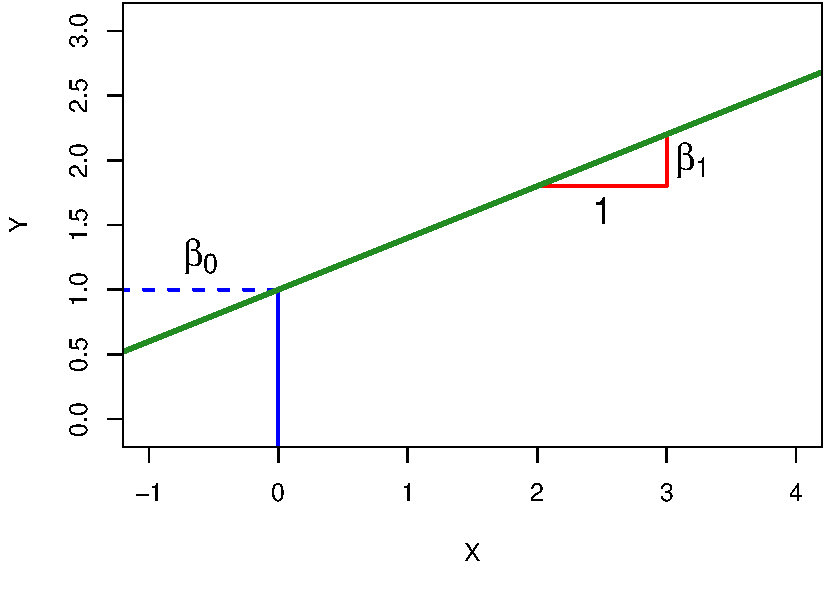
\includegraphics[width=0.7\textwidth]{03-linear-models_files/figure-beamer/linear-regression-schematic-1} \end{center}

\end{frame}

\begin{frame}{Linear regression}

We estimate the two unknown parameters in the model using a procedure
known as \alert{least squares}, where we minimise the
\alert{Residual Sum of Squares}
\(\mathrm{RSS} = \sum_{i=1}^n \varepsilon_i\)

\begin{center}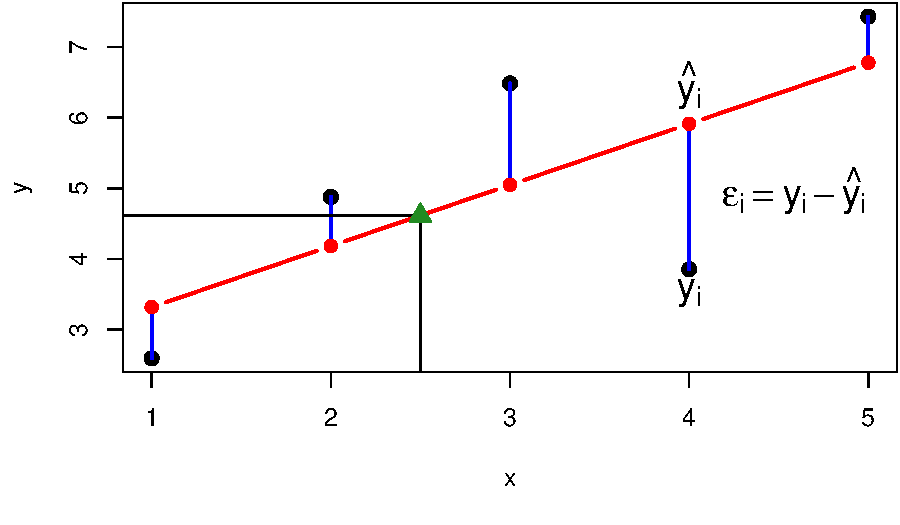
\includegraphics[width=0.7\linewidth]{03-linear-models_files/figure-beamer/linear-reg-least-squares-1} \end{center}

\end{frame}

\begin{frame}{Linear regression}

Estimates of parameters (\(\beta_j\)) are for the \emph{population}
based on the fit to our \emph{sample} of data

\begin{center}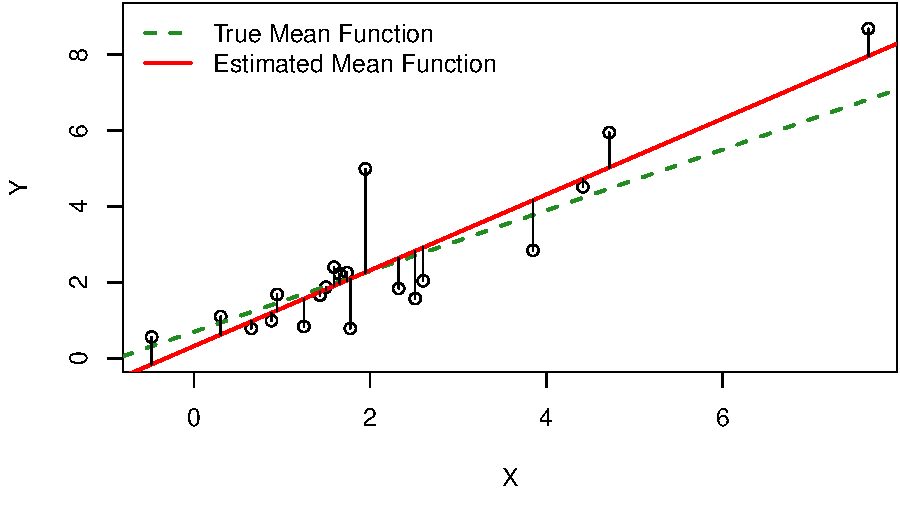
\includegraphics[width=0.7\linewidth]{03-linear-models_files/figure-beamer/true-versus-estimate-line-1} \end{center}

\end{frame}

\begin{frame}{Linear regression}

Data were 20 observations generated from the following model

\[y_i = 0.7 + 0.8x_i + \varepsilon_i \;\;\;\; \varepsilon_i \sim N(\mu = 0, \sigma = 1)\]

Fitted model estimates are: \(\hat{\beta}_0\) = 0.32 and
\(\hat{\beta}_1\) = 0.999

The parameters are means \& the uncertainty in the estimated values is
captured by their standard errors

Confidence intervals for the estimates:

\begin{itemize}
\tightlist
\item
  \(\beta_0 \pm t_{0.975} \mathrm{SE}_{\beta_0}\) = -0.401, 1.041
\item
  \(\beta_1 \pm t_{0.975} \mathrm{SE}_{\beta_1}\) = 0.741, 1.256
\end{itemize}

\end{frame}

\begin{frame}{Ventricular shortening \& Diabetes}

Example data are from a study of the effects of blood glucose levels on
heart function in diabetes patients

\begin{center}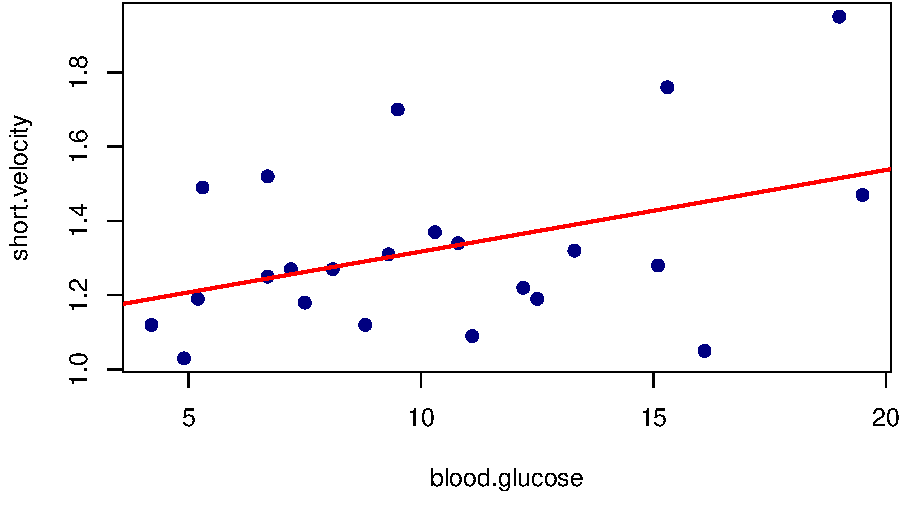
\includegraphics[width=0.7\linewidth]{03-linear-models_files/figure-beamer/thuesen-example-1} \end{center}

\end{frame}

\begin{frame}[fragile]{Ventricular shortening \& Diabetes: Model
summary}

\scriptsize

\begin{verbatim}

Call:
lm(formula = short.velocity ~ blood.glucose, data = thuesen)

Residuals:
     Min       1Q   Median       3Q      Max 
-0.40141 -0.14760 -0.02202  0.03001  0.43490 

Coefficients:
              Estimate Std. Error t value Pr(>|t|)    
(Intercept)    1.09781    0.11748   9.345 6.26e-09 ***
blood.glucose  0.02196    0.01045   2.101   0.0479 *  
---
Signif. codes:  0 '***' 0.001 '**' 0.01 '*' 0.05 '.' 0.1 ' ' 1

Residual standard error: 0.2167 on 21 degrees of freedom
  (1 observation deleted due to missingness)
Multiple R-squared:  0.1737,    Adjusted R-squared:  0.1343 
F-statistic: 4.414 on 1 and 21 DF,  p-value: 0.0479
\end{verbatim}

\normalsize

\end{frame}

\begin{frame}[fragile]{Ventricular shortening \& Diabetes: Model
summary}

\scriptsize

\begin{verbatim}
              Estimate Std. Error t value Pr(>|t|)    
(Intercept)    1.09781    0.11748   9.345 6.26e-09 ***
blood.glucose  0.02196    0.01045   2.101   0.0479 *  
---
Signif. codes:  0 '***' 0.001 '**' 0.01 '*' 0.05 '.' 0.1 ' ' 1
\end{verbatim}

\normalsize

\begin{itemize}
\tightlist
\item
  \texttt{Estimate} column contains the estimated parameters
\item
  The intercept is 1.098, the ventricular shortening velocity (VSV) at a
  blood glucose level of 0 mmol/L
\item
  For every increase of 1 mmol/L glucose in blood, VSV \emph{increases}
  by 0.022
\item
  Each row in the table is a statistical test of a parameter, with a
  null hypothesis \(\beta_j\) = 0
\item
  \(t\) is the \alert{test statistic} for the test
  \(t_j = \frac{\beta_j - 0}{\mathrm{SE}_{\beta_j}}\)
\item
  \emph{What is the probability of observing a value as extreme as
  \(\hat{\beta}_j\) if \(\beta_j\) = 0?}
\item
  \emph{Is the observed coefficient expected if there was no
  relationship between \(x\) and \(y\)}
\end{itemize}

\end{frame}

\begin{frame}{T tests}

\(n\) - 2 degrees of freedom = 21

If \(t\) statistic lies in either rejection regions, reject
H\textsubscript{0} at \(\alpha\) = 0.05 level

\begin{center}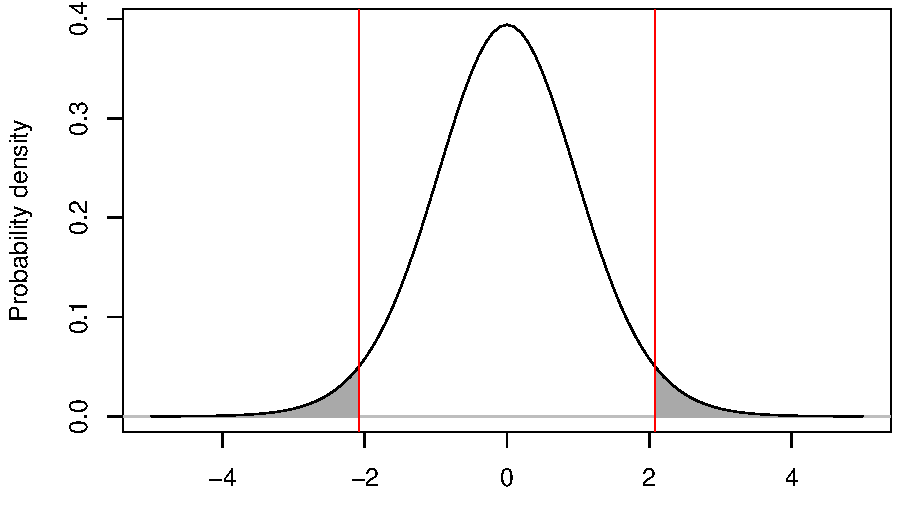
\includegraphics[width=0.7\linewidth]{03-linear-models_files/figure-beamer/rejection-regions-plot-1} \end{center}

\end{frame}

\begin{frame}[fragile]{ANOVA table}

Linear regression can be seen as a partitioning of variance in the data
in amounts explained by variables in the model \& unexplained variance

\alert{Mean squares} can only be positive; even a variable unrelated to
response will explain some variance

Compare the ratio of Mean square (the SSq normalised by degrees of
freedom) with an \emph{F} distribution with 1 \& 21 degrees of freedom

\scriptsize

\begin{verbatim}
Analysis of Variance Table

Response: short.velocity
              Df Sum Sq Mean Sq F value Pr(>F)  
blood.glucose  1  0.207   0.207    4.41  0.048 *
Residuals     21  0.986   0.047                 
---
Signif. codes:  0 '***' 0.001 '**' 0.01 '*' 0.05 '.' 0.1 ' ' 1
\end{verbatim}

\normalsize

\end{frame}

\begin{frame}{ANOVA table}

\(F\) is the \(F\)-ratio, the ratio of the regression and residual
variances

\[F = \frac{\sum\limits^n_{i=1}(\hat{y}_i - \bar{y})^2 / p}{\sum\limits^n_{i=1}(y_i - \hat{y}_i)^2 / [n-(p+1)]} = \frac{\mathrm{MS_{reg}}}{\mathrm{MS_{resid}}}\]

Probability of \(F\) greater than or equal to observed from
\(F\)-distribution with \(p\) and \(n - (p + 1)\) degrees of freedom

\end{frame}

\begin{frame}{ANOVA table}

Large values of \emph{F} are evidence against the null hypothesis of no
relationship

Reference distribution is \(\mathsf{F_{1,21}}\); all rejection region is
in upper tail

\begin{center}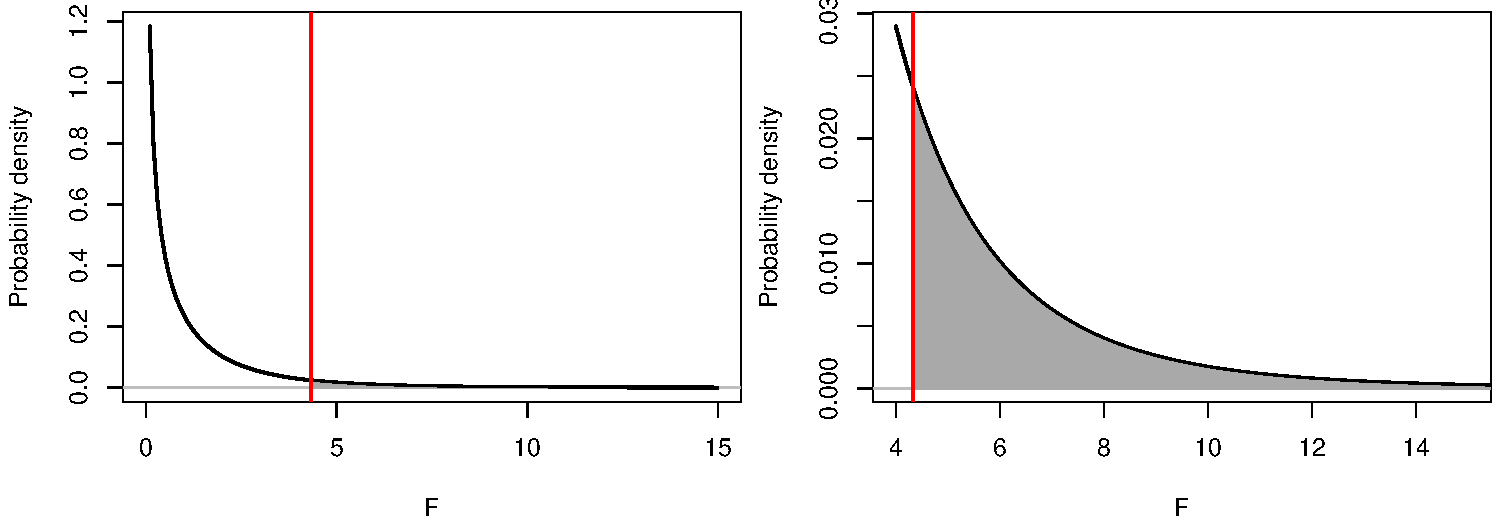
\includegraphics[width=\textwidth]{03-linear-models_files/figure-beamer/F-rejection-regions-plot-1} \end{center}

\end{frame}

\begin{frame}{R-Squared}

\(R^2\) is a commonly reported measure of variance explained by the
regression

\(R^2\) is the \alert{coefficient of determination}, the ratio of the
variance explained to the total variance

\[R^2 = \frac{\mathrm{SS_{reg}}}{\mathrm{SS_{reg} + RSS}} = 1 - \frac{\mathrm{SS_{resid}}}{\mathrm{SS_{total}}}\]

One problem with \(R^2\) is that increases as you add predictors to the
model even if those predictors have no explanatory power

\end{frame}

\begin{frame}{Adjusted R-squared}

Adjusted \(R^2\) takes into account number of predictors in the model

\[R^2_{\mathrm{adj}} = 1 - \frac{\mathrm{SS_{resid}} / [n - (p + 1)]}{\mathrm{SS_{total}} / (n-1)}\]

Neither measure is a particularly \emph{useful} summary; don't indicate
how the regression model will predict new observations

The \alert{effect size}, the size of the model coefficients, is far more
useful

\end{frame}

\section{Assumptions of the linear
model}\label{assumptions-of-the-linear-model}

\begin{frame}{Assumptions of the linear model}

To fit the model, we don't need to make any assumptions, beyond
linearity

\alert{Statistical inference} on the estimated parameters depends on a
number of assumptions

\begin{enumerate}
\def\labelenumi{\arabic{enumi}.}
\tightlist
\item
  The linear model correctly describes the functional relationship
  between \(y\) and \(x\)
\item
  The \(x_i\) are measured without error
\item
  For any given value of \(x_i\), the sampled \(y_i\) values are
  \alert{independent} with normally distributed errors
\item
  Variances are constant along the regression line/model
\end{enumerate}

\end{frame}

\begin{frame}{Assumptions of the linear model I}

\textbf{The linear model correctly describes the functional relationship
between \(y\) and \(x\)}

Effectively, this assumption is about whether the model we've fitted
represents the true underlying relationship between \(x\) and \(y\)

\emph{Is the relationship well approximated via a straight line?}

\emph{Would a curved line (\alert{polynomial}) be better?}

If we have the model form wrong, our model will be \alert{biased};
fitted values different appreciably from the true values

If violated the estimate of predictor variances (\(\sigma^2\)) will be
inflated

Incorrect model specification can show itself as patterns in the
residuals

\end{frame}

\begin{frame}{Assumptions of the linear model I}

\begin{center}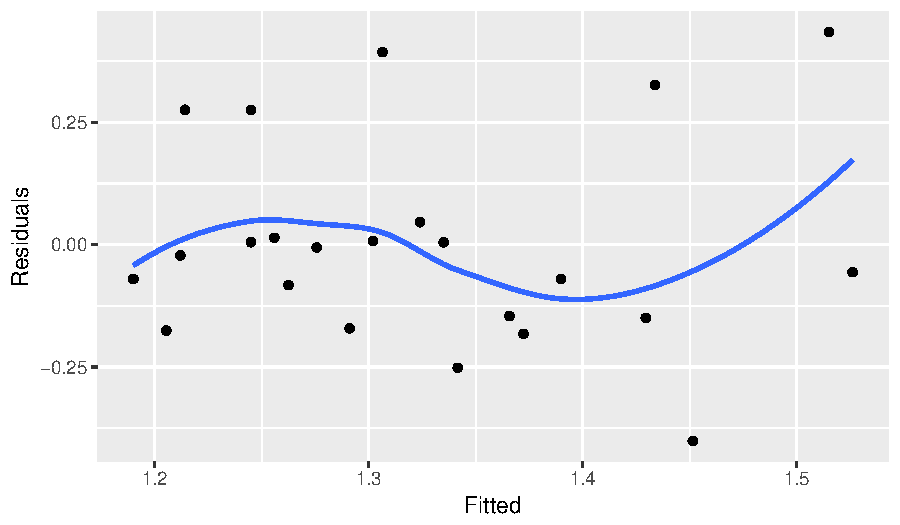
\includegraphics[width=0.7\linewidth]{03-linear-models_files/figure-beamer/resid-vs-fitted-1} \end{center}

\end{frame}

\begin{frame}{Assumptions of the linear model II}

\textbf{\(x_i\) are measured without error}

This assumption states that we know the values of the predictor
variable(s) \(x\) \emph{exactly}

Allows us to isolate the error component (\(\varepsilon_i\)) as random
variation in \(y\)

Estimates \(\hat{\beta}_j\) will be biased if there is error in \(x\)

This is often ignored in data analysis, but modern, advanced approaches
can account for this extra source of variation

\end{frame}

\begin{frame}{Assumptions of the linear model III}

\textbf{For any \(x_i\), the sampled \(y_i\) are \alert{independent}
with normally distributed errors}

\textbf{Variances are constant along the regression line/model}

These 2 assumptions relate to distribution of the residuals
(\(\varepsilon_i\)), or, \emph{conditional upon} the values of \(x\), of
\(y\)

\(\varepsilon_i\) are assumed to follow a \alert{Normal} distribution
with zero mean and constant variance

Independence and normality of errors allows us to use parametric theory
for confidence intervals and hypothesis tests on the \(F\)-ratio.

Allows a single constant variance \(\sigma^2\) for the variance of the
regression line/model

Each residual is drawn from the same distribution; Normal with mean
zero, variance \(\hat{\sigma}^2\)

Non-constant variances can be recognised through plots of residuals
(among others); residuals get wider as the values of \(y\) increase

\end{frame}

\begin{frame}{Assumptions of the linear model III}

\begin{center}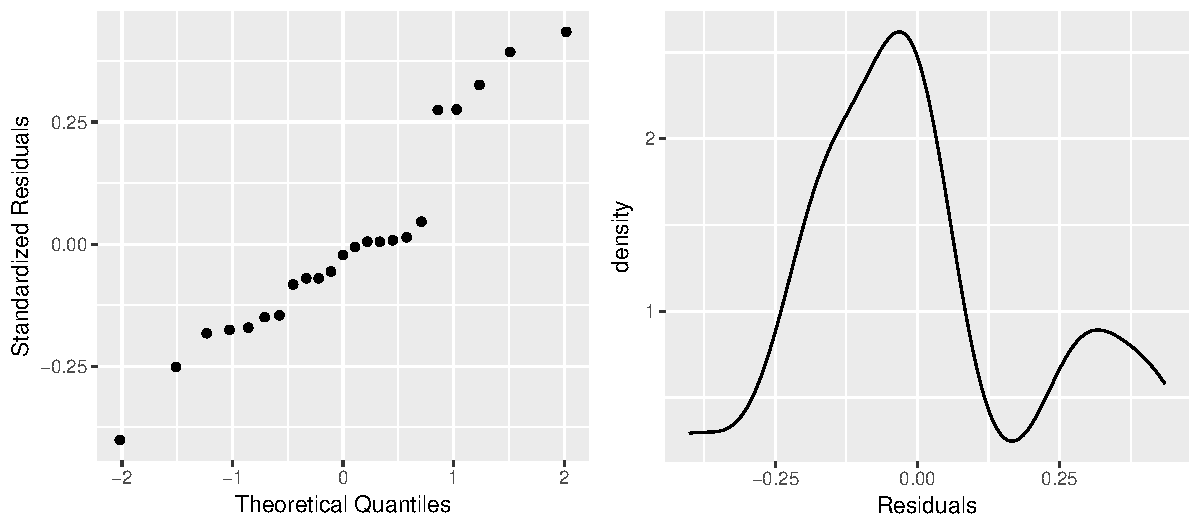
\includegraphics[width=0.9\textwidth]{03-linear-models_files/figure-beamer/svmod-qqplot-1} \end{center}

\end{frame}

\begin{frame}{Assumptions of the linear model III}

\begin{center}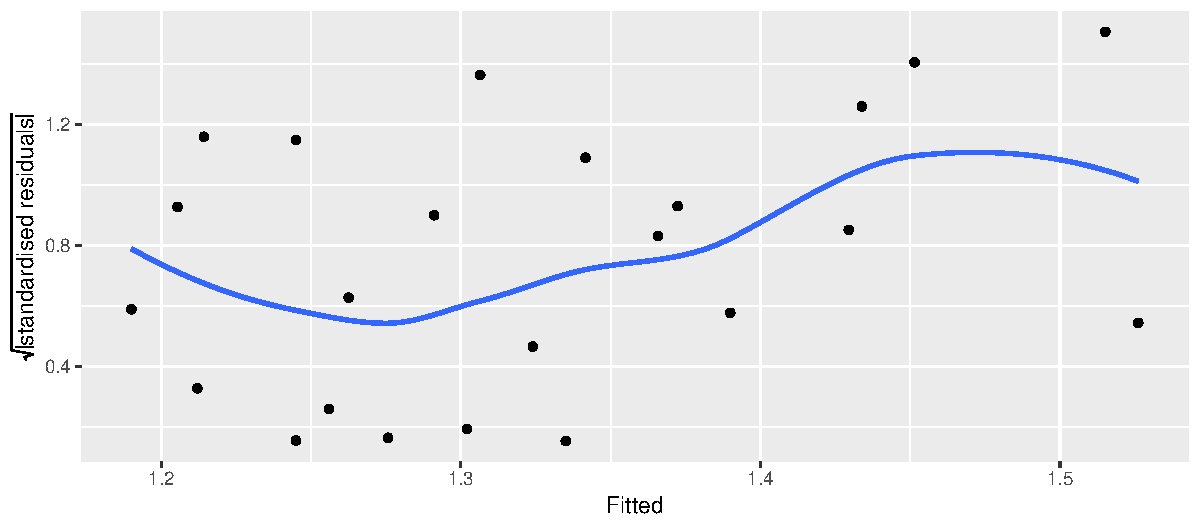
\includegraphics[width=0.9\textwidth]{03-linear-models_files/figure-beamer/svmod-scale-location-plot-1} \end{center}

\end{frame}

\begin{frame}{Assumptions of the linear model IV}

\alert{Independence} is a key assumption; knowing the value of one
residual tells use nothing about another

Data that have spatial or temporal components, or represent repeated
observations on the same set of individuals are commonly encountered \&
violate this assumption

\end{frame}

\section{Outliers, Leverage \&
Influence}\label{outliers-leverage-influence}

\begin{frame}{Outliers, Leverage \& Influence}

An \alert{outlier} is an observation which is inconsistent with the rest
of a sample

An observation can be an outlier due to the response variable(s) or one
or more of the predictor variables having values outside their expected
limits

An outlier may also result from: incorrect measurement, incorrect data
entry, transcription error, recording error

Two main concepts

\begin{itemize}
\tightlist
\item
  \alert{Leverage}: Potential for an outlier to be influential
\item
  \alert{Influence}: Observation is influential if its deletion
  substantially changes the results
\end{itemize}

\end{frame}

\begin{frame}{Outliers, Leverage \& Influence}

\alert{Leverage} measures the degree to which individual observations
affect the the fitted value for that observation

Leverage values are also known as \alert{hat values}, as they are the
values on the diagonal of the \emph{hat matrix}, which projects the
observed values onto the fitted values of the model

Hat matrix is so called because it puts a \alert{hat on} \(\mathbf{Y}\):
\(\mathbf{\hat{Y} = HY}\)

Leverage ranges from 1/n to 1

Observation has high leverage if its hat value is 2--3 times the average
hat value: \(h = (p+1)/n\), where \(p+1\) is number of coefficients
(inc. the intercept)

\end{frame}

\begin{frame}{Outliers, Leverage \& Influence}

\begin{center}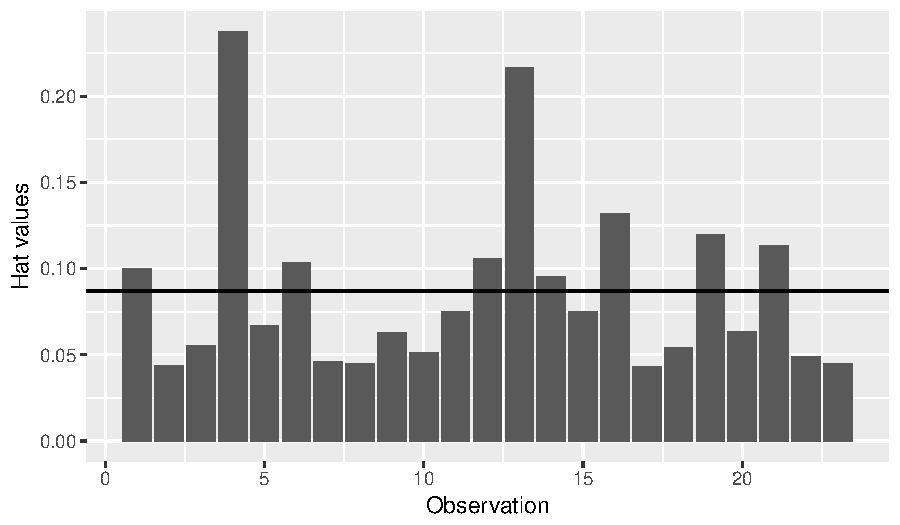
\includegraphics[width=0.7\linewidth]{03-linear-models_files/figure-beamer/svmod-hatvalues-plot-1} \end{center}

\end{frame}

\begin{frame}{Outliers, Leverage \& Influence}

An observation that combines \emph{outlyingness} with high leverage
exerts an \alert{influence} on the estimated regression coefficients

If an influential observation is deleted from the model, the
\emph{estimated coefficients change substantially}

\(\mathsf{dfbeta}_{ij}\) assesses the impact on the \(j\)th coefficient
of deleting the \(i\)th observation

\[\mathsf{dfbeta}_{ij} = \beta_{j(-i)} - \beta_j\]

The \(\mathsf{dfbeta}_{ij}\) are expressed in the metric of the
coefficient

A standardised version, \(\mathsf{dfbetas}_{ij}\) divides
\(\mathsf{dfbeta}_{ij}\) by the standard error of \(\beta_j\)

Influential observations have
\(\mathsf{dfbetas}_{ij} \geq 2 / \sqrt{n}\)

\end{frame}

\begin{frame}{Outliers, Leverage \& Influence: Cook's Distance}

One problem with \(\mathsf{dfbetas}_{ij}\) is that there are so many
numbers!

One for each observation for every \(\beta_j\): \(n \times (p+1)\)

\alert{Cook's Distance}, \(D_i\), is a scale invariant measure of
distance between \(\beta_j\) and \(\beta_{j(-i)}\)

\[D_i = \frac{e^2_i}{s^2(p+1)} \times \frac{h_i}{1-h_i}\]

where \(e_i^2\) is the squared residual \& \(h_i\) is the hat value for
\(x_i\); \(s^2\) is the variance of the residuals

The first fraction is a measure of \alert{outlyingness}, the second of
\alert{leverage}

\(D_i \geq 4 / (n - p - 1)\) suggested as a cutoff for high values of
\(D_i\)

\end{frame}

\begin{frame}{Outliers, Leverage \& Influence: Cook's Distance}

\begin{center}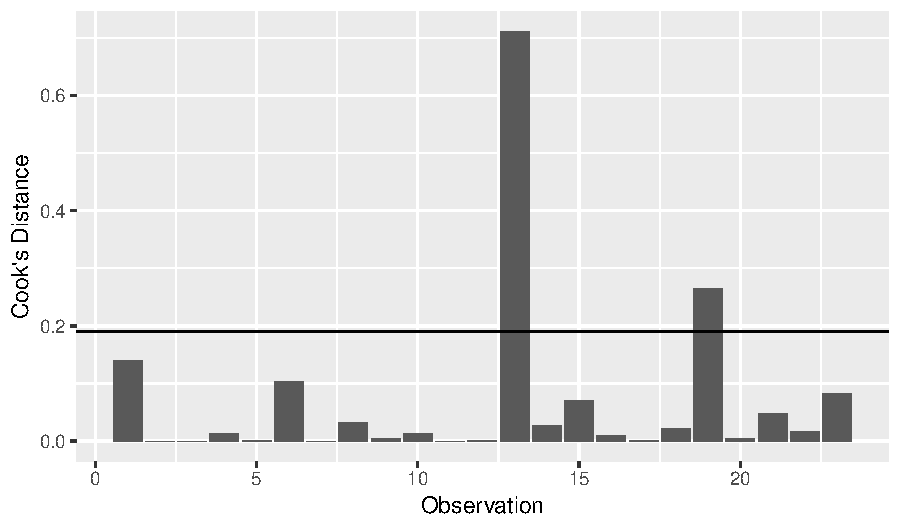
\includegraphics[width=0.7\linewidth]{03-linear-models_files/figure-beamer/svmod-cooks-distance-plot-1} \end{center}

\end{frame}

\begin{frame}{Outliers, Leverage \& Influence: Example}

\begin{center}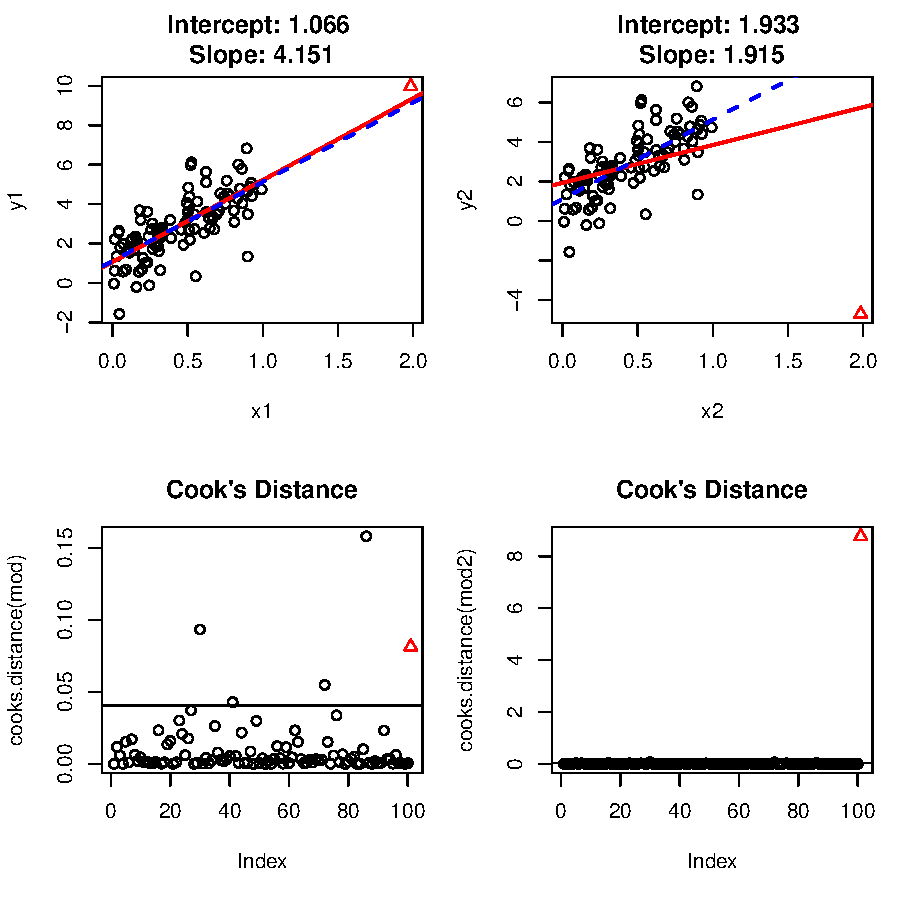
\includegraphics[width=0.5\textwidth]{03-linear-models_files/figure-beamer/leverge-influence-example-1} \end{center}

\end{frame}

\section{Multiple Regression}\label{multiple-regression}

\begin{frame}{Multiple regression}

The simple regression model readily generalises to the situation where
we have \(m\) predictors not just one
\[y_i = \beta_0 + \beta_1x_{i1} + \beta_2x_{i2} + \dots + \beta_mx_{im} + \varepsilon_i\]

Now we have \(m + 1\) parameters to estimate, one for intercept and one
each for the \(m\) predictors \(x_m\). Can have as many as \(m = n - 1\)
predictor variables

Simple description as a regression lines starts to be blurred; with
\(m = 2\) we have a \emph{regression plane}

But in other respects the model fitting, assumptions, etc remain the
same

We do now have the problem of deciding which of the \(m\) predictions
are related to \(y\)

\end{frame}

\begin{frame}[fragile]{Multiple regression: lung function in cystic
fibrosis patients}

\texttt{pemax} is \emph{maximal expiratory pressure}, a measure of lung
function

A number of predictor variables thought to affect \texttt{pemax}

\begin{itemize}
\tightlist
\item
  Age, sex, height, weight, \& body mass (\texttt{bmp}) of each patient
\item
  Forced expiratory (\texttt{fev1}) \& residual (\texttt{rv}) volume
\item
  Functional residual capacity (\texttt{frc}) \& total lung capacity
  (\texttt{tlc})
\end{itemize}

\end{frame}

\begin{frame}[fragile]{Multiple regression: lung function in cystic
fibrosis patients}

Typical statistical output for the full model

\tiny

\begin{verbatim}

Call:
lm(formula = pemax ~ age + sex + height + weight + bmp + fev1 + 
    rv + frc + tlc, data = cystfibr)

Residuals:
   Min     1Q Median     3Q    Max 
-37.34 -11.53   1.08  13.39  33.41 

Coefficients:
            Estimate Std. Error t value Pr(>|t|)
(Intercept)  176.058    225.891    0.78     0.45
age           -2.542      4.802   -0.53     0.60
sexFemale     -3.737     15.460   -0.24     0.81
height        -0.446      0.903   -0.49     0.63
weight         2.993      2.008    1.49     0.16
bmp           -1.745      1.155   -1.51     0.15
fev1           1.081      1.081    1.00     0.33
rv             0.197      0.196    1.00     0.33
frc           -0.308      0.492   -0.63     0.54
tlc            0.189      0.500    0.38     0.71

Residual standard error: 25.5 on 15 degrees of freedom
Multiple R-squared:  0.637, Adjusted R-squared:  0.42 
F-statistic: 2.93 on 9 and 15 DF,  p-value: 0.032
\end{verbatim}

\normalsize

\end{frame}

\begin{frame}[fragile]{Multiple regression: lung function in cystic
fibrosis patients}

No \emph{t} tests are significant, but this is only a reflection of what
would happen if you removed that variable from model leaving others in
the model

However, the joint \emph{F} test is significant, indicating that there
is an effect in there somewhere

\scriptsize

\begin{verbatim}
Analysis of Variance Table

Model 1: pemax ~ 1
Model 2: pemax ~ age + sex + height + weight + bmp + fev1 + rv + frc + 
    tlc
  Res.Df   RSS Df Sum of Sq     F Pr(>F)  
1     24 26833                            
2     15  9731  9     17101 2.929  0.032 *
---
Signif. codes:  0 '***' 0.001 '**' 0.01 '*' 0.05 '.' 0.1 ' ' 1
\end{verbatim}

\normalsize

\end{frame}

\begin{frame}[fragile]{Multiple regression: lung function in cystic
fibrosis patients}

\alert{Sequential sums of squares} (Type I), ordering matters \& changes
results

\scriptsize

\begin{verbatim}
Analysis of Variance Table

Response: pemax
          Df Sum Sq Mean Sq F value Pr(>F)   
age        1  10098   10098  15.566 0.0013 **
sex        1    955     955   1.473 0.2437   
height     1    155     155   0.239 0.6321   
weight     1    632     632   0.975 0.3392   
bmp        1   2862    2862   4.412 0.0530 . 
fev1       1   1549    1549   2.388 0.1431   
rv         1    562     562   0.866 0.3668   
frc        1    195     195   0.300 0.5920   
tlc        1     92      92   0.142 0.7112   
Residuals 15   9731     649                  
---
Signif. codes:  0 '***' 0.001 '**' 0.01 '*' 0.05 '.' 0.1 ' ' 1
\end{verbatim}

\normalsize

\end{frame}

\section{Model selection}\label{model-selection}

\begin{frame}{Model selection}

Where we have several candidate covariates for inclusion in a model, we
face the problem of selecting a \alert{minimal, adequate model}

A minimal, adequate model is one that is complex enough to provide
sufficient fit to the observed response but no more complex than is
necessary

Several automated techniques available to help

\small

\begin{enumerate}
\def\labelenumi{\arabic{enumi}.}
\tightlist
\item
  Best subsets regression
\item
  Forward selection
\item
  Backwards elimination
\item
  Stepwise regression (forward selection and backward elimination)
\end{enumerate}

\normalsize

Regardless of method used to select a minimal model there's no free
lunch

\emph{p} values from tests on the selected model do not account for the
selection procedure; anti-conservative, too many variables selected

\end{frame}

\begin{frame}{Model selection}

Model or subset selection often used for 2 reasons

\begin{enumerate}
\def\labelenumi{\arabic{enumi}.}
\item
  \alert{Interpretation}: Smaller subset of predictors with strongest
  effects on response \(y\) may be easier to interpret and explain
\item
  \alert{Prediction accuracy}: least squares estimates have low
  \textbf{bias} but large \textbf{variance}

  Can sometimes improve prediction accuracy by shrinking the
  coefficients or setting some to zero. In doing so we sacrifice a bit
  of \textbf{bias}
\end{enumerate}

Subset selection leads to a small set of interpretable predictors, with
possibly lower error (MSE) than the full model

Subset selection is a discrete process --- predictors are either
\emph{in} the model, or \emph{not}

\end{frame}

\begin{frame}{Information Criteria I}

\alert{Akaike information criterion} (AIC) is an index of fit that takes
account of the parsimony of the model by penalising the number of
parameters

The more parameters in the model the better the fit --- if you have as
many parameters as data points then the fit is perfect but the model has
no explanatory power! A Trade-off

AIC is useful as it explicitly penalises any superfluous parameters in
the model by adding \(2p\) to the variance or deviance of the model

\[\mathrm{AIC} = -2 \times \log(\mathrm{likelihood}) + 2p\]

Associated is Bayes information criterion (BIC), which applies a
stronger penalty of \(p \log n\), where \(n\) is number of observations

For linear regression the \(-2 \times \log(\mathrm{likelihood})\) is
\(n \log(RSS/n) + \mathrm{constant}\)

\end{frame}

\begin{frame}{Information Criteria II}

We can use AIC and BIC to compare two or more \alert{nested} models

Nested means that one model is a subset of the other

The model with the \emph{smallest} AIC or BIC is to be preferred

Note that you can get negative values for AIC and BIC. This is fine,
just go for the smallest value: -21.5 is better than -15.4

Difference in AIC of 2 is expected with a redundant parameter. Models
with AIC differing by 2 or less are effectively the same

\end{frame}

\begin{frame}{Best subsets}

\alert{Best subsets} identifies the \emph{best} model of each
\emph{size}, \& compare models via a statistic; \alert{AIC} and
\alert{BIC} are commonly used

\begin{center}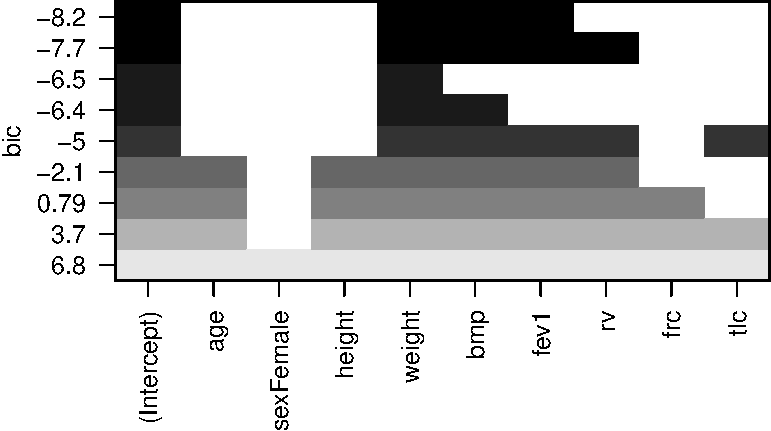
\includegraphics[width=0.7\linewidth]{03-linear-models_files/figure-beamer/best-subsets-1} \end{center}

\end{frame}

\begin{frame}{Best subsets}

Having some manual control is handy; might want to remove the other lung
function variables first

\begin{center}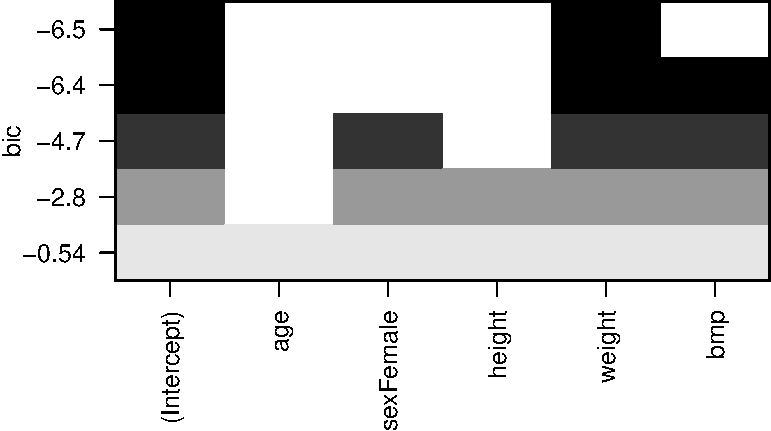
\includegraphics[width=0.7\linewidth]{03-linear-models_files/figure-beamer/best-subsets-2-1} \end{center}

\end{frame}

\begin{frame}{Forwards, backwards, and stepwise selection}

\alert{Stepwise selection} is a combination of \textbf{forward}
selection \& \textbf{backward} elimination steps

\alert{Forward selection}

\begin{enumerate}
\def\labelenumi{\arabic{enumi}.}
\tightlist
\item
  Start with only the constant term
\item
  Fit \(m\) models, each adding one of the \(m\) predictors to the
  current model
\item
  Identify the \emph{best} model from the set of models
\item
  Add the predictor from this \emph{best} model to the current model
  \textbf{if} this results in a significant improvement in model fit
\item
  Repeat 3--4 until no further addition results in a better model
\end{enumerate}

\end{frame}

\begin{frame}[fragile]{Forward selection}

\alert{Forward selection} starts with only the intercept term \& adds
variables until no improvement can be made

AIC used to assess improvement as terms added; notice that the inclusion
of \texttt{rv} is probably unwarranted

\scriptsize

\begin{verbatim}
      Step Df  Deviance Resid. Df Resid. Dev      AIC
1          NA        NA        24   26832.64 176.4625
2 + weight -1 10827.159        23   16005.48 165.5453
3    + bmp -1  1914.939        22   14090.54 164.3596
4   + fev1 -1  2552.354        21   11538.19 161.3635
5     + rv -1  1183.588        20   10354.60 160.6578
\end{verbatim}

\normalsize

\end{frame}

\begin{frame}[fragile]{Backwards elimination}

\alert{Backwards elimination} starts with the full model \& removes
variables until no improvement can be made

Can only fit the full model if you have fewer variables than
observations

\scriptsize

\begin{verbatim}
      Step Df  Deviance Resid. Df Resid. Dev      AIC
1          NA        NA        15   9731.250 169.1055
2    - sex  1  37.90214        16   9769.152 167.2027
3    - tlc  1 115.94265        17   9885.094 165.4977
4    - frc  1 133.15598        18  10018.250 163.8322
5    - age  1 145.33646        19  10163.587 162.1923
6 - height  1 191.01331        20  10354.600 160.6578
\end{verbatim}

\begin{verbatim}

Call:
lm(formula = pemax ~ weight + bmp + fev1 + rv, data = cystfibr)

Coefficients:
(Intercept)       weight          bmp         fev1           rv  
    63.9467       1.7489      -1.3772       1.5477       0.1257  
\end{verbatim}

\normalsize

\end{frame}

\begin{frame}[fragile]{Stepwise selection}

Stepwise selection starts with either the intercept or the full model \&
adds or removes variables at each step until no improvement can be made

\scriptsize

\begin{verbatim}
      Step Df  Deviance Resid. Df Resid. Dev      AIC
1          NA        NA        24   26832.64 176.4625
2 + weight -1 10827.159        23   16005.48 165.5453
3    + bmp -1  1914.939        22   14090.54 164.3596
4   + fev1 -1  2552.354        21   11538.19 161.3635
5     + rv -1  1183.588        20   10354.60 160.6578
\end{verbatim}

\begin{verbatim}

Call:
lm(formula = pemax ~ weight + bmp + fev1 + rv, data = cystfibr)

Coefficients:
(Intercept)       weight          bmp         fev1           rv  
    63.9467       1.7489      -1.3772       1.5477       0.1257  
\end{verbatim}

\normalsize

\end{frame}

\begin{frame}{Stepwise selection}

Here AIC used to assess improvement, but often \emph{p} values \& formal
statistical tests are used to test improvement

Multiple testing is then a major problem, but AIC may be too liberal

No guarantee that selection will find the best model or that they will
agree on the best model

\emph{p} values of terms in the selected models no longer have their
usual meaning

Model coefficients (\(\hat{\beta}_j\)) are biased

\end{frame}

\section{Interactions}\label{interactions}

\begin{frame}{Interaction terms}

Up to now we've only considered the \alert{main effects} of the
variables in our model

There, terms are \alert{additive}, each variable contributing an amount
to the model irrespective of the values of the other predictors

But what if the effect of one variable depends upon the value of one or
more other variables?

This is where \alert{interaction terms} come in

\end{frame}

\begin{frame}{Interaction terms}

Two explanatory variables \alert{interact} when the \alert{partial}
effect of one depends on the \emph{value} of the other

\textbf{\alert{Marginal effect}} --- effect of \(x_1\) on \(y\)
\emph{ignoring} the effects on \(y\) of the other variables \(x_j\)

\textbf{\alert{Partial effect}} --- effect of \(x_1\) on \(y\)
\emph{accounting for} the effects on \(y\) of the other variables
\(x_j\)

Interactions occur in several types

\begin{itemize}
\tightlist
\item
  continuous --- factor interactions
\item
  continuous --- continuous interactions
\item
  factor --- factor interactions
\end{itemize}

\end{frame}

\begin{frame}{Interaction Terms: Continuous---factor interactions}

\begin{block}{PTSD in adult female survivors of childhood sexual abuse}

45 women treated at a clinic who reported childhood sexual abuse (CSA)
were measured for PTSD \& childhood physical abuse (CPA) on standardised
scales

31 women at same clinic but did not report CSA were also assessed

Two models

\begin{equation}
\mathsf{PTSD}_i = \beta_0 + \beta_1 \mathsf{CSA}_i + \beta_2 \mathsf{CPA}_i + \varepsilon_i
\end{equation}

\begin{equation}
\mathsf{PTSD}_i = \beta_0 + \beta_1 \mathsf{CSA}_i + \beta_2 \mathsf{CPA}_i + \beta_3 (\mathsf{CSA}_i \times \mathsf{CPA}_i) \varepsilon_i
\end{equation}

\end{block}

\end{frame}

\begin{frame}{Interaction Terms: Continuous---factor interactions}

\begin{block}{PTSD in adult female survivors of childhood sexual abuse}

\begin{center}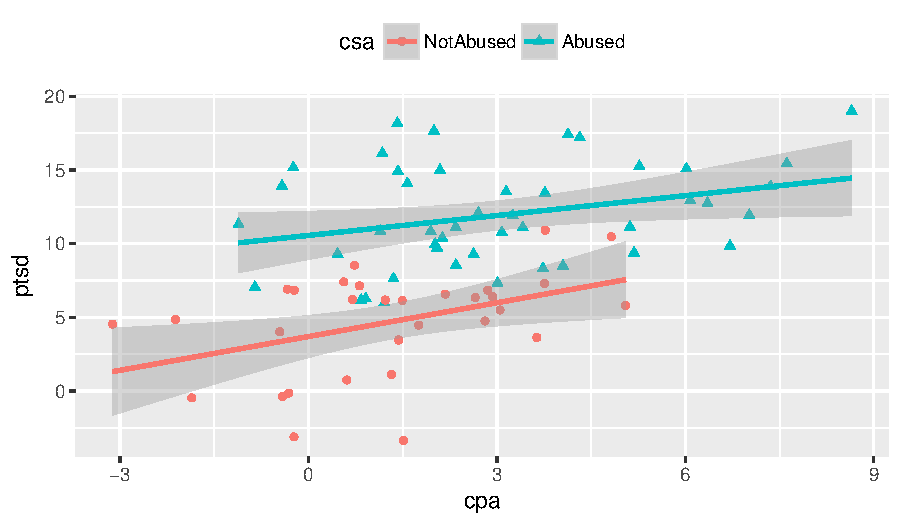
\includegraphics[width=0.7\linewidth]{03-linear-models_files/figure-beamer/sex-abuse-plot-1} \end{center}

\end{block}

\end{frame}

\begin{frame}[fragile]{Interaction Terms: Continuous---factor
interactions}

\scriptsize

\begin{verbatim}

Call:
lm(formula = ptsd ~ cpa * csa, data = sexab)

Residuals:
    Min      1Q  Median      3Q     Max 
-8.1999 -2.5313 -0.1807  2.7744  6.9748 

Coefficients:
              Estimate Std. Error t value Pr(>|t|)    
(Intercept)     3.6959     0.7107   5.201 1.79e-06 ***
cpa             0.7640     0.3038   2.515   0.0142 *  
csaAbused       6.8612     1.0747   6.384 1.48e-08 ***
cpa:csaAbused  -0.3140     0.3685  -0.852   0.3970    
---
Signif. codes:  0 '***' 0.001 '**' 0.01 '*' 0.05 '.' 0.1 ' ' 1

Residual standard error: 3.279 on 72 degrees of freedom
Multiple R-squared:  0.5828,    Adjusted R-squared:  0.5654 
F-statistic: 33.53 on 3 and 72 DF,  p-value: 1.133e-13
\end{verbatim}

\normalsize

\end{frame}

\begin{frame}[fragile]{Interaction Terms: Continuous---factor
interactions}

Interactions between factors can be represented as \alert{dummy}
variables, indicating group/combination membership

Reference level (\texttt{NotAbused}) absorbed into the intercept term

Model is parameterised in terms of differences of means from the
reference level

\scriptsize

\begin{verbatim}
  (Intercept)      cpa csaAbused cpa:csaAbused
1           1  2.04786         1       2.04786
2           1  0.83895         1       0.83895
3           1 -0.24139         1      -0.24139
\end{verbatim}

\begin{verbatim}
   (Intercept)      cpa csaAbused cpa:csaAbused
74           1 -1.85753         0             0
75           1  2.85253         0             0
76           1  0.81138         0             0
\end{verbatim}

\normalsize

\end{frame}

\begin{frame}{Interaction Terms: Continuous---factor interactions}

Model fits \emph{with} interaction

\begin{center}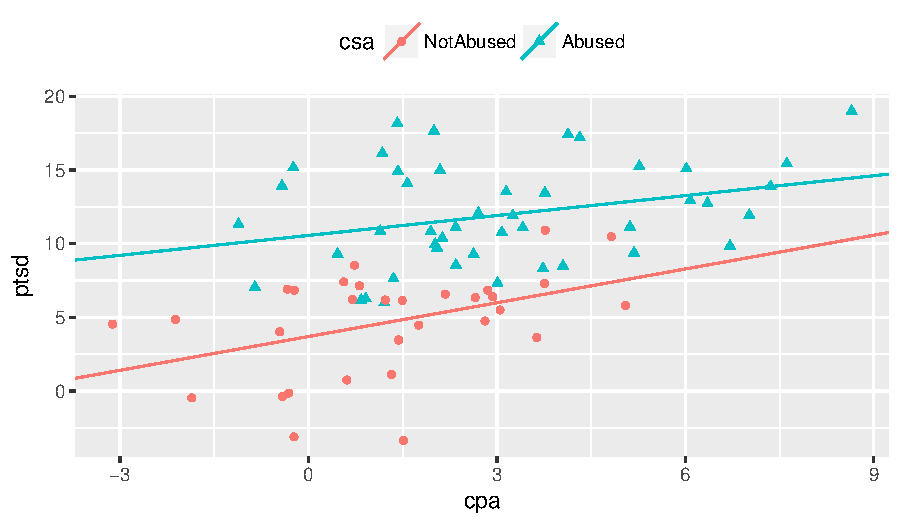
\includegraphics[width=0.7\linewidth]{03-linear-models_files/figure-beamer/sex-abuse-plot-interaction-model-1} \end{center}

\end{frame}

\begin{frame}{Interaction Terms: Continuous---factor interactions}

Model fits \emph{without} interaction

\begin{center}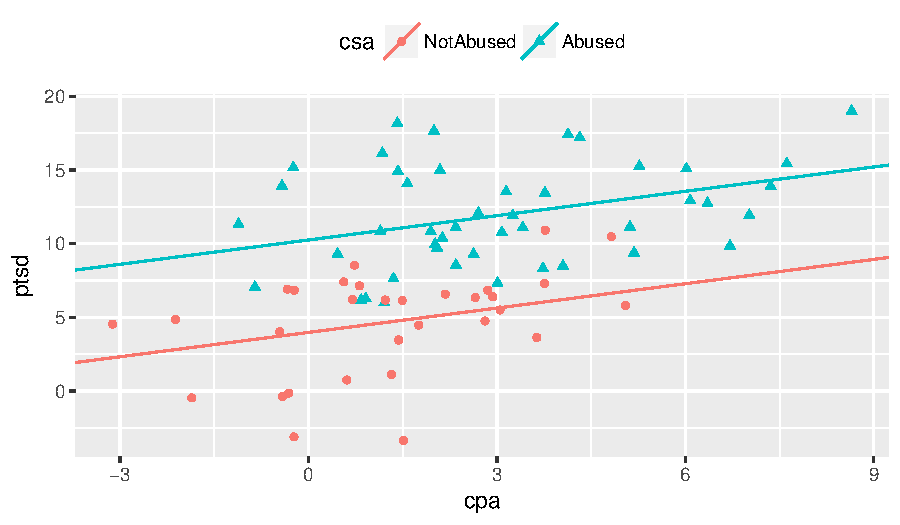
\includegraphics[width=0.7\linewidth]{03-linear-models_files/figure-beamer/sex-abuse-plot-additive-model-1} \end{center}

\end{frame}

\begin{frame}{Interaction Terms: Continuous---continuous interactions}

In continuous---continuous interactions we don't need to worry about
coding

This type of interaction is represented by a new variable that is the
product of the two variables

If we have \(x_1\) and \(x_2\), the interaction would be be
\((x_1 \times x_2)\)

\end{frame}

\begin{frame}{Interaction Terms: Continuous---continuous interactions}

50 infants of age approximately 2 months were weighed immediately before
\& after each breast feeding

Measured the intake of breast milk (dL) along with various other data

\begin{center}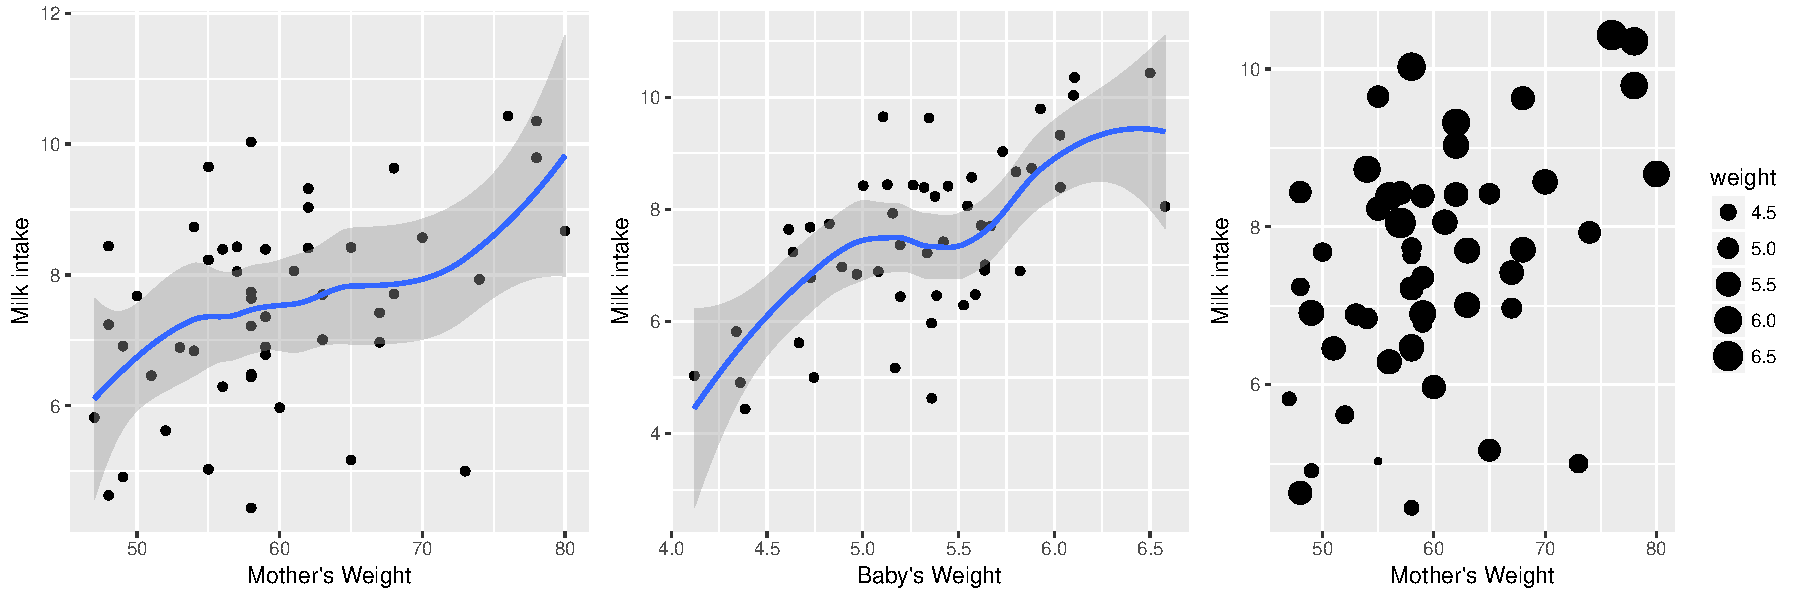
\includegraphics[width=\textwidth]{03-linear-models_files/figure-beamer/kfm-data-1} \end{center}

\end{frame}

\begin{frame}[fragile]{Interaction Terms: Continuous---continuous
interactions}

\scriptsize

\begin{verbatim}

Call:
lm(formula = dl.milk ~ mat.weight * weight, data = kfm)

Residuals:
     Min       1Q   Median       3Q      Max 
-2.45005 -0.73689  0.09775  0.80987  2.67499 

Coefficients:
                  Estimate Std. Error t value Pr(>|t|)  
(Intercept)       15.68279   10.79790   1.452   0.1532  
mat.weight        -0.27868    0.18354  -1.518   0.1358  
weight            -1.89188    1.99057  -0.950   0.3469  
mat.weight:weight  0.05797    0.03340   1.736   0.0893 .
---
Signif. codes:  0 '***' 0.001 '**' 0.01 '*' 0.05 '.' 0.1 ' ' 1

Residual standard error: 1.13 on 46 degrees of freedom
Multiple R-squared:  0.4755,    Adjusted R-squared:  0.4413 
F-statistic:  13.9 on 3 and 46 DF,  p-value: 1.389e-06
\end{verbatim}

\normalsize

\end{frame}

\begin{frame}[fragile]{Interaction Terms: Continuous---continuous
interactions}

Testing whether the interaction term is required via an \emph{F} test

Marginally significant; effect looks small

\scriptsize

\begin{verbatim}
Analysis of Variance Table

Model 1: dl.milk ~ mat.weight + weight
Model 2: dl.milk ~ mat.weight * weight
  Res.Df    RSS Df Sum of Sq      F  Pr(>F)  
1     47 62.562                              
2     46 58.716  1    3.8456 3.0128 0.08931 .
---
Signif. codes:  0 '***' 0.001 '**' 0.01 '*' 0.05 '.' 0.1 ' ' 1
\end{verbatim}

\normalsize

\end{frame}

\begin{frame}{Interaction Terms: Continuous---continuous interactions}

Visualisation of the effect of continuous---continuous interactions

\begin{center}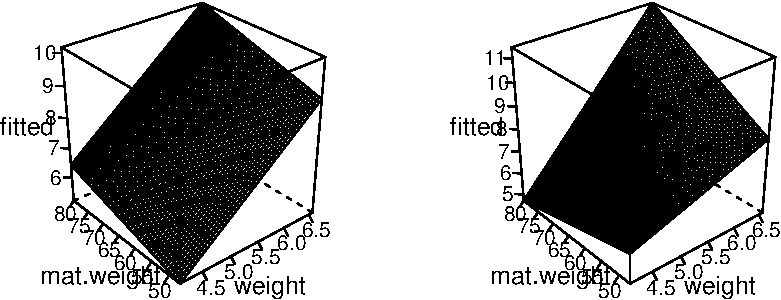
\includegraphics[width=0.9\textwidth]{03-linear-models_files/figure-beamer/kfm-wireframe-1} \end{center}

\end{frame}

\begin{frame}{Interaction Terms: Effects displays}

Focus on high-order terms in the model; each high-order term is allowed
to vary over it's range, while other variables are held at some average
values

\begin{center}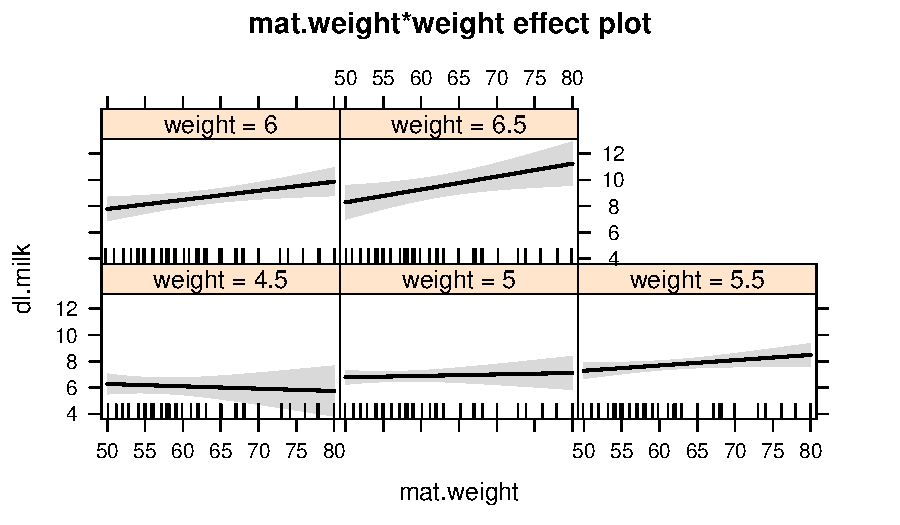
\includegraphics[width=0.7\linewidth]{03-linear-models_files/figure-beamer/kfm-effects-1} \end{center}

\end{frame}

\begin{frame}{Interaction terms: Principal of Marginality}

The \emph{partial} (\emph{main}) effects of variables in a model are
\alert{marginal} to any interaction terms in which they participate

Partial effects of CPA \& CSA are \emph{marginal} to the
\(\mathsf{CPA} \times \mathsf{CSA}\) interaction

In general, should not test partial effects that are marginal to an
interaction term

Can test the partial effects if we can remove the interaction on
empirical or theoretical grounds

Also doesn't make sense to fit models with interaction terms without
including the main effects of terms participating in the interaction

\end{frame}

\section{Analysis of Variance}\label{analysis-of-variance}

\begin{frame}{Analysis of Variance}

\alert{Analysis of Variance} (ANOVA) is the classic name for a linear
model where the predictor (explanatory) variables are \emph{categorical}

Earlier ANOVA used to partition variance in \(y\) into components
explained by \(x_j\) \& a residual component not explained by the
regression model

A slightly more restricted view of ANOVA is that it is a technique for
partitioning the variation in \(y\) into that explained by one or more
categorical predictor variables

The categories of each factor are the groups or experimental treatments

\end{frame}

\begin{frame}{Analysis of Variance}

ANOVA considers the different sources of variation that might arise on a
data set

Of particular interest is on the differences in the mean value of \(y\)
between groups

We can think of \emph{within-group} and \emph{between-group} variances

\begin{itemize}
\tightlist
\item
  \textbf{Between-group} variance is that due to the treatment (group)
  effects
\item
  \textbf{Within-group} variance is that due to the variability of
  individuals \& measurement error
\end{itemize}

There Will always be variation between individuals but is this
within-group variance large or small, relative to the variance
\emph{between} groups?

\end{frame}

\begin{frame}{ANOVA how \emph{many} ways?}

One of the complications surrounding ANOVA is the convoluted
nomenclature used describe variants of the method

Variants commonly distinguished by the number of categorical variables
in the model

\begin{itemize}
\tightlist
\item
  \alert{One-way ANOVA} contains a single categorical variable
\item
  \alert{Two-way ANOVA} contains two categorical variables
\item
  \alert{Three-way ANOVA} contains three categorical variables
\item
  \ldots{}
\end{itemize}

Two-way and higher ANOVA potentially involve the consideration of
\emph{factor---factor} interactions

\end{frame}

\begin{frame}[fragile]{One-way ANOVA}

In a \alert{One-way ANOVA} we have a single categorical variable \(x\)
with \emph{two or more} levels With two levels we have the same analysis
as the \emph{t} test

If we consider differences between patients with different illnesses, we
might use an \texttt{illness-group} factor whose \emph{levels} might be

\begin{itemize}
\tightlist
\item
  Multiple Sclerosis,
\item
  Irritable Bowel Syndrome, \&
\item
  Chronic Fatigue Syndrome
\end{itemize}

If we're testing the 5 doses of a drug on Multiple Sclerosis patients,
the factor might be \texttt{dose} with levels: placebo, 5 mg, 10 mg, 15
mg, \& 20 mg

\end{frame}

\begin{frame}{One-way ANOVA}

Assume we have a single categorical variable \(x\) with three levels.
The One-way ANOVA model using dummy coding or treatment contrasts is

\[y_i = \beta_0 + \beta_1D_{i1} + \beta_2D_{i2} + \varepsilon_i\]

Where \(D_{ij}\) is the coding for the \(j\)th level (group) for the
\(i\)th observation

\begin{longtable}[]{@{}ccc@{}}
\toprule
Group & \(D_1\) & \(D_2\)\tabularnewline
\midrule
\endhead
1 & 0 & 0\tabularnewline
2 & 1 & 0\tabularnewline
3 & 0 & 1\tabularnewline
\bottomrule
\end{longtable}

\end{frame}

\begin{frame}{One-way ANOVA}

Measure the \textbf{between-group} variance as the \emph{regression sums
of squares}

The \textbf{within-group} variance is the \emph{residual sums of
squares}

An \textbf{omnibus test} F statistic is used to test the null hypothesis
of \emph{no differences among population group means}

\[\mathsf{H_0:} \; \beta_1 = \beta_2 = 0\]

\end{frame}

\begin{frame}{One-way ANOVA}

Attree \& colleagues (2003, \emph{Applied Neurophysiology}
\textbf{10}(2)) conducted a study of variation in cognitive function in
patients with \emph{Inflammatory Bowel Disease} (IBD) \& \emph{Irritable
Bowel Syndrome} (IBS) relative to health \alert{controls} (Healthy)

Response variable was the \emph{Verbal IQ Score} (VIQ)

Previous studies had shown that VIQs were impaired in other patient
groups relative to healthy controls

\end{frame}

\begin{frame}{One-way ANOVA}

\begin{center}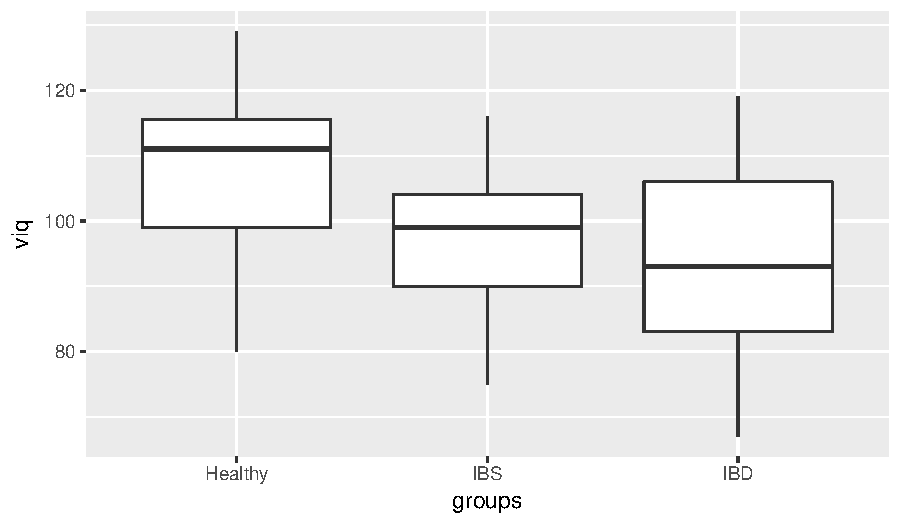
\includegraphics[width=0.7\linewidth]{03-linear-models_files/figure-beamer/verbal-1-1} \end{center}

\end{frame}

\begin{frame}[fragile]{One-way ANOVA}

Results of fitting one-way ANOVA to the verbal IQ score data

\scriptsize

\begin{verbatim}
Analysis of Variance Table

Response: viq
          Df  Sum Sq Mean Sq F value    Pr(>F)    
groups     2  3365.4 1682.70  11.403 4.103e-05 ***
Residuals 85 12543.5  147.57                      
---
Signif. codes:  0 '***' 0.001 '**' 0.01 '*' 0.05 '.' 0.1 ' ' 1
\end{verbatim}

\normalsize

\end{frame}

\begin{frame}{One-way ANOVA}

Multiple comparisons

\begin{center}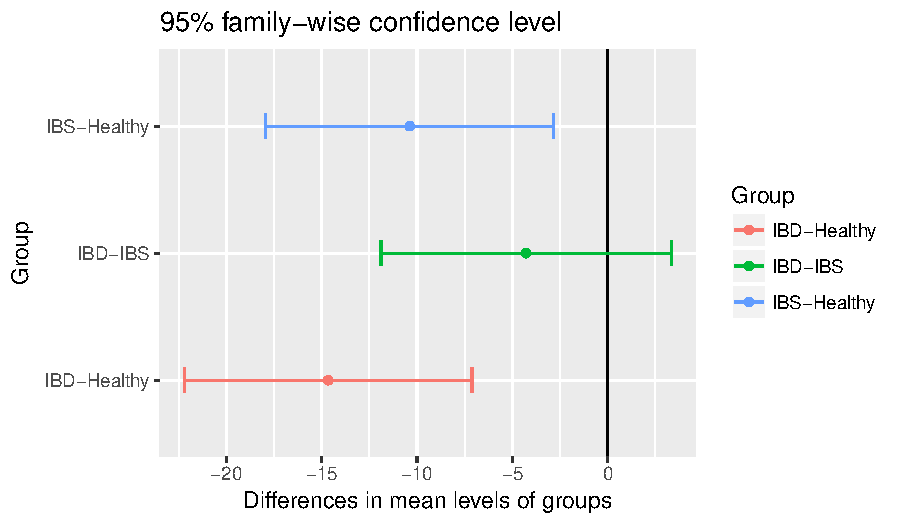
\includegraphics[width=0.7\linewidth]{03-linear-models_files/figure-beamer/verbal-2-plot-1} \end{center}

\end{frame}

\section{Example}\label{example}

\begin{frame}{PCBs in Lake Trout}

Human exposure to polychlorinated biphenyls (PCBs) from consumption of
fish is a health concern in the Great Lakes region of the US

\begin{itemize}
\tightlist
\item
  Exposure limits based on fish tissue concentrations; anglers can not
  easily determine this concentration
\item
  Can size of fish be used to infer PCB tissue concentration?
\item
  Data are PCB concentrations in lake trout (1974--2003)
\end{itemize}

\end{frame}

\begin{frame}[fragile]{PCBs in Lake Trout}

\begin{Shaded}
\begin{Highlighting}[]
\NormalTok{laketrout <-}\StringTok{ }\KeywordTok{read.csv}\NormalTok{(}\StringTok{"../00-data-sets/laketrout2.csv"}\NormalTok{)}
\NormalTok{## gets rid of a very small pcb value and a length 0 fish}
\NormalTok{laketrout <-}\StringTok{ }\KeywordTok{with}\NormalTok{(laketrout, laketrout[pcb>}\KeywordTok{exp}\NormalTok{(-}\DecValTok{2}\NormalTok{) &}\StringTok{ }\NormalTok{length>}\DecValTok{0}\NormalTok{, ])}
\KeywordTok{ggplot}\NormalTok{(laketrout, }\KeywordTok{aes}\NormalTok{(}\DataTypeTok{x =} \NormalTok{length, }\DataTypeTok{y =} \KeywordTok{log}\NormalTok{(pcb))) +}
\StringTok{    }\KeywordTok{geom_point}\NormalTok{() +}
\StringTok{    }\KeywordTok{geom_smooth}\NormalTok{(}\DataTypeTok{colour =} \StringTok{"forestgreen"}\NormalTok{, }\DataTypeTok{se =} \OtherTok{FALSE}\NormalTok{, }\DataTypeTok{size =} \FloatTok{1.5}\NormalTok{) +}
\StringTok{    }\KeywordTok{geom_smooth}\NormalTok{(}\DataTypeTok{method =} \StringTok{"lm"}\NormalTok{, }\DataTypeTok{colour =} \StringTok{"red"}\NormalTok{, }\DataTypeTok{se =} \OtherTok{FALSE}\NormalTok{, }\DataTypeTok{size =} \FloatTok{1.5}\NormalTok{) +}
\StringTok{    }\KeywordTok{theme_bw}\NormalTok{()}
\end{Highlighting}
\end{Shaded}

\begin{center}\includegraphics[width=0.6\textwidth]{03-linear-models_files/figure-beamer/lake-trout-0-1} \end{center}

\end{frame}

\begin{frame}[fragile]{Lake trout PCB example}

\scriptsize

\begin{verbatim}

Call:
lm(formula = log(pcb) ~ length, data = laketrout)

Residuals:
     Min       1Q   Median       3Q      Max 
-1.74263 -0.52741 -0.06745  0.40549  2.47294 

Coefficients:
             Estimate Std. Error t value Pr(>|t|)    
(Intercept) -2.132082   0.165622  -12.87   <2e-16 ***
length       0.123398   0.006602   18.69   <2e-16 ***
---
Signif. codes:  0 '***' 0.001 '**' 0.01 '*' 0.05 '.' 0.1 ' ' 1

Residual standard error: 0.7673 on 629 degrees of freedom
  (15 observations deleted due to missingness)
Multiple R-squared:  0.3571,    Adjusted R-squared:  0.3561 
F-statistic: 349.4 on 1 and 629 DF,  p-value: < 2.2e-16
\end{verbatim}

\normalsize

\end{frame}

\begin{frame}[fragile]{Lake trout PCB example}

\begin{itemize}
\tightlist
\item
  \emph{Estimate} is \(\beta_j\), the model coefficients, on log scale
\item
  For 1 cm increase in fish length, PCB tissue concentration increases
  by \(\mathrm{1.3 \, mg \, kg^{-1}}\)
\item
  \emph{t-value} is the \(t\) statistic, the ratio of the estimate and
  its standard error \[t = \frac{\hat{\beta}_j}{\hat{\mathrm{se}}_j}\]
\item
  Probability of achieving a \(t\) as large or larger than the observed
\item
  Intercept of no biological interest --- PCB concentration of a length
  0 fish
\end{itemize}

\scriptsize

\begin{verbatim}
(Intercept)      length 
 -2.1320818   0.1233985 
\end{verbatim}

\normalsize

\end{frame}

\begin{frame}[fragile]{Lake trout PCB example}

\begin{itemize}
\tightlist
\item
  \(F\) is the \(F\)-ratio, the ratio of the regression and residual
  variances
  \[F = \frac{\sum\limits^n_{i=1}(\hat{y}_i - \bar{y})^2 / p}{\sum\limits^n_{i=1}(y_i - \hat{y}_i)^2 / [n-(p+1)]} = \frac{\mathrm{MS_{reg}}}{\mathrm{MS_{resid}}}\]
\item
  Probability of \(F\) greater than or equal to observed from
  \(F\)-distribution with \(p\) and \(n - (p + 1)\) degrees of freedom
\end{itemize}

\scriptsize

\begin{Shaded}
\begin{Highlighting}[]
\KeywordTok{anova}\NormalTok{(pcb.m1)}
\end{Highlighting}
\end{Shaded}

\begin{verbatim}
Analysis of Variance Table

Response: log(pcb)
           Df Sum Sq Mean Sq F value    Pr(>F)    
length      1 205.70 205.703   349.4 < 2.2e-16 ***
Residuals 629 370.31   0.589                      
---
Signif. codes:  0 '***' 0.001 '**' 0.01 '*' 0.05 '.' 0.1 ' ' 1
\end{verbatim}

\normalsize

\end{frame}

\begin{frame}{Re-use}

Copyright © (2015) Gavin L. Simpson Some Rights Reserved

Unless indicated otherwise, this slide deck is licensed under a
\href{http://creativecommons.org/licenses/by/4.0/}{Creative Commons
Attribution 4.0 International License}.

\begin{center}
  \ccby
\end{center}

\end{frame}

\end{document}
